\begin{figure}
	\centering
	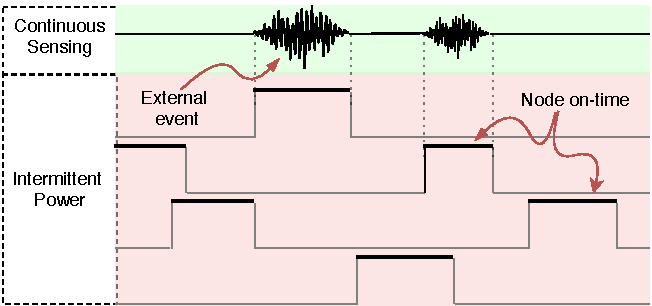
\includegraphics[width=\columnwidth]{figures/coalInterSen}
	\caption{\fullsys (\sys) is a group of intermittently powered sensory nodes that sense continuously despite the intermittent power supply. \sys exploits the inherent randomization of energy harvesting systems or enforce artificial randomization to preserve an efficient and continuous sensing functionality.}
	\label{fig:powerCycle}
\end{figure}

The Internet of Things is the engine that will drive smart cities. In these cities, cars will not need to wait in front of traffic lights for non-existing pedestrians to cross the road; doors, upon leaving, will provide people with weather forecast; and jackets will adjust air circulation based on body temperature. Smart cities will gain their awareness through billions of sensors.

Batteries do not provide a viable solution to power all the sensors, in smart cities. Batteries may be bulky, for example, 32\% of a $\SI{1}{g}$ sensing "backpack" fixed on a cyborg insect is a battery~\cite{daly2010pulsed}; hazardous; and expensive---they may deplete and require servicing devices that are otherwise fully functional. Moreover, the raw materials for making batteries are also limited. Therefore, future sensors must leave batteries behind and rely on perpetual energy sources. 

Natural energy sources such as light, vibration, and heat can power tiny sensors directly~\cite{margolies2016panda, gorlatova2014movers, gorlatova2010energy, gollakota2014emergence,}. Tiny energy harvesters, however, can only scavenge a very limited power from such energy sources~\cite{liu2013ambient}. Therefore, an energy-harvesting sensor operates intermittently. An intermittent sensor starts by harvesting a certain amount of energy in its buffer (i.e. a super-capacitor). Then, it triggers operation which depletes the buffered energy quickly, as the power consumption rate tends to be much higher than the power accumulation rate. Once the energy is below a certain level, the sensor experience a complete power-down, the cycle of charging and operating continues indefinitely~\cite{colin2018reconfigurable}.

Intermittent devices trade-off a reliable energy source (the battery) for sustainable---when a large number of sensors are considered---energy source, ambient energy. This trade-off generates many challenges~\cite{lucia2017intermittent}. For example, preserving computation progress under frequent power interrupts, enabling timely operations with indeterminate power-down duration, and the fact that nodes operate intermittently. 

Many of these challenges have been tackled. For example, \cite{lucia2017intermittent,mementos,dino,colin2016chain,balsamo2015hibernus} studied the intermittent computation problem, which is concerned with the preservation of an application progress and memory integrity under frequent power failures; \cite{hester2017timely} investigated the timely operation challenge, which is concerned with data freshness after a power interrupt; and \cite{yildirim2018ink, samoyed_pldi_2019} introduced the event-driven execution for the intermittent domain, which is concerned with input and output operations under arbitrarily-timed power loss.% However, all previous work has considered the intermittency as an inherent characteristic of these systems and have not attempted to control it. 

Despite the significant progress that has been achieved in the intermittent domain, \textit{the system availability problem} has not been addressed. A monitoring sensor that has a very low probability to be available when an external event occurs is not worth deploying. A sensor that is capable of capturing only very short events has a limited number of potential applications (imagine that you want to control room lights with a batteryless microphone. The microphone is capable of processing a single word. If you say "on" lights turned on but other systems might start to operate also---a specification problem. If you say "light" to eliminate other systems you lose the ability to control the light---a functionality problem). Consequently, intermittent sensors have not gained widespread adoption. 

This paper tackles the paradox of continuous sensing on intermittent devices. It studies the randomized power cycle of energy-harvesting platforms and makes a key observation about the inter-relationship between these platforms. Building on top of this observation, it introduces a new type of sensors that we call \textit{\fullsys} (\sys). The \sys is defined as the abstraction of a group of energy-aware intermittent nodes. This paper provides intermittent nodes with a software-based tool for intermittent timing and ambient energy estimation. It, then, identifies four different \sys powering states and investigates the side effects of the overpowering states. Finally, it introduces a \fullcim---a prototype of a \sys--- and summaries the results of various tests. 

This paper makes several key contributions:
\begin{itemize}
		\item We introduce a new type of sensor that is an intermittently powered but senses continuously. \textit{\fullsys} (\sys) is the abstraction of a group of intermittently powered sensors. It uses natural energy sources not only for power but also to distribute its intermittent nodes uniformly in time.
		\item We model the \sys availability and back up our model with reasoning and validate it against in-the-wild measured data and under controllable energy conditions.   
		\item We introduce an algorithm for intermittent timing. It enables intermittent nodes to self time their power-downs duration, without requiring extra hardware. 
		\item We show how an intermittent node can exploit the tight relationship between the operation time and the ambient energy to estimate the number of its active counterparts.
		\item We study the effect of varying the energy harvesting conditions on the \sys and identify four \sys powering states: under-powered, intermittently powered, hibernating, continuously powered. Then, we show how favorable energy conditions can degrade the \sys performance.
		\item We prototype \fullsys in a form of \fullcim. Voice control is a convenient interface for a human to interact with miniaturized devices. Moreover, it enables us to easily study the behavior of the \sys under a different type of external events (i.e. bursty arrival of events). 
\end{itemize}

\todo{Potential applications, relocate to the appreciated location}
 For example, once a certain on/off cycle is preserved, an intermittent wake-up receiver can be implemented; an intermittent acoustic monitoring system for monitoring engines modules---the sound produced by a deformed gear tooth---can be made. Moreover, with the advances in passive communication (such as passive light~\cite{}, and backscatter tag-to-tag~\cite{liu2013ambient} communication) battery-free miniaturized sensors can form self-powered wireless sensor network to, for instance, create smart wallpaper and revolutionize smart buildings. 

